\documentclass[english]{beamer}
\usepackage{makeidx}
\usepackage{color}
\usepackage{graphicx}
\usetheme{Goettingen}
\setbeamercovered{transparent}

\usenavigationsymbolstemplate{}
\AtBeginSection[]{
  \frame<beamer>{
    \frametitle{Next...}
    \tableofcontents[currentsection]
   }
}

\definecolor{ListingBorderColor}{gray}{0.55}
\definecolor{ListingBackgroundColor}{gray}{0.95}

\usepackage{babel}
\usepackage{hyperref}
\usepackage{enumerate}
\usepackage{enumerate}
\usepackage{longtable}
\usepackage[T1]{fontenc}
\usepackage{ucs}
\usepackage[latin1]{inputenc}
\usepackage{textcomp}
\usepackage{alltt}
\usepackage{listings}

\title{Git the basics}
\author{Bart Trojanowski, \href{mailto:bart@jukie.net}{bart@jukie.net}}
\institute{Jukie Networks Inc.}
\date{July 9th, 2008}

\setcounter{tocdepth}{2}


\newcommand{\mysection}[2]{
  \hypertarget{#2}{}
  \section{#1}
  \label{#2}
}
\newcommand{\mysubsection}[2]{
  \hypertarget{#2}{}
  \subsection{#1}
  \label{#2}
}

\definecolor{code-black}{rgb}{0,0,0}
\definecolor{code-green}{rgb}{0,0.3,0}
\definecolor{code-orange}{rgb}{0.4,0.3,0}
\definecolor{code-blue}{rgb}{0,0,0.5}
\definecolor{code-gray}{rgb}{0.7,0.7,0.7}
\definecolor{code-white}{rgb}{1,1,1}
\newcommand{\ttt}[1]{
  \texttt{\textcolor{code-black}{#1}}
}
\newcommand{\CMD}[1]{
  \texttt{\textcolor{code-green}{#1}}
}
\newcommand{\cmd}[1]{
  \texttt{\textcolor{code-orange}{#1}}
}
\newcommand{\gui}[1]{
  \texttt{\textcolor{code-blue}{#1}}
}
\newcommand{\faint}[1]{
  \texttt{\textcolor{code-gray}{#1}}
}
\newcommand{\hide}[1]{
  \texttt{\textcolor{code-white}{#1}}
}

\newcommand{\GitCmdTable}[4]{
{\tiny \tt
\begin{tabular}{llll}
#2{add}              & #4{fast-export}       & #4{merge-one-file} & #3{revert}             \\
#3{am}               & #4{fast-import}       & #4{merge-resolve}  & #2{rm}                 \\
#3{annotate}         & #2{fetch}             & #4{merge-subtree}  & #3{send-email}         \\
#3{apply}            & #4{fetch-pack}        & #4{merge-tree}     & #4{send-pack}          \\
#4{archimport}       & #4{filter-branch}     & #1{mergetool}      & #4{sh-setup}           \\
#3{archive}          & #4{fmt-merge-msg}     & #4{mktag}          & #1{shell}              \\
#2{bisect}           & #4{for-each-ref}      & #4{mktree}         & #3{shortlog}           \\
#2{blame}            & #3{format-patch}      & #2{mv}             & #2{show}               \\
#2{branch}           & #4{fsck}              & #4{name-rev}       & #3{show-branch}        \\
#3{bundle}           & #4{fsck-objects}      & #4{pack-objects}   & #4{show-index}         \\
#4{cat-file}         & #2{gc}                & #4{pack-redundant} & #4{show-ref}           \\
#4{check-attr}       & #4{get-tar-commit-id} & #4{pack-refs}      & #2{stash}              \\
#4{check-ref-format} & #2{grep}              & #4{parse-remote}   & #2{status}             \\
#2{checkout}         & #1{gui}               & #4{patch-id}       & #4{stripspace}         \\
#4{checkout-index}   & #4{hash-object}       & #4{peek-remote}    & #2{submodule}          \\
#3{cherry}           & #4{http-fetch}        & #4{prune}          & #3{svn}                \\
#3{cherry-pick}      & #4{http-push}         & #4{prune-packed}   & #4{symbolic-ref}       \\
#1{citool}           & #4{imap-send}         & #2{pull}           & #2{tag}                \\
#2{clean}            & #4{index-pack}        & #2{push}           & #4{tar-tree}           \\
#2{clone}            & #2{init}              & #3{quiltimport}    & #4{unpack-file}        \\
#2{commit}           & #4{init-db}           & #4{read-tree}      & #4{unpack-objects}     \\
#4{commit-tree}      & #3{instaweb}          & #2{rebase}         & #4{update-index}       \\
#2{config}           & #2{log}               & #4{receive-pack}   & #4{update-ref}         \\
#4{count-objects}    & #4{lost-found}        & #3{reflog}         & #3{update-server-info} \\
#4{cvsexportcommit}  & #4{ls-files}          & #4{relink}         & #4{upload-archive}     \\
#4{cvsimport}        & #4{ls-remote}         & #2{remote}         & #4{upload-pack}        \\
#4{cvsserver}        & #4{ls-tree}           & #4{repack}         & #4{var}                \\
#4{daemon}           & #4{mailinfo}          & #4{repo-config}    & #4{verify-pack}        \\
#3{describe}         & #4{mailsplit}         & #4{request-pull}   & #4{verify-tag}         \\
#2{diff}             & #2{merge}             & #4{rerere}         & #3{whatchanged}        \\
#4{diff-files}       & #4{merge-base}        & #2{reset}          & #4{write-tree}         \\
#4{diff-index}       & #4{merge-file}        & #4{rev-list}       &                        \\
#4{diff-tree}        & #4{merge-index}       & #4{rev-parse}      & #1{gitk}               \\
\end{tabular}
}}

\begin{document}
% =====================================================================
\label{header}\hypertarget{header}{}
\frame{\maketitle}

% ---------------------------------------------------------------------
\begin{frame}
        \frametitle{Table of contents}
        \par\noindent
        \tableofcontents
\end{frame}

% =====================================================================
% =====================================================================
\mysection{Concepts}{_concepts}
% ---------------------------------------------------------------------
\begin{frame}
\frametitle{Concepts}
\begin{itemize}
        \item Source Control Management
                \begin{itemize}
                        \item track changes to files
                        \item repository / database of changes
                        \item working directory / current state
                \end{itemize}

        \pause{}
        \item Centralized SCM
                \begin{itemize}
                        \item server: single database
                        \item client: working directory \&{} state
                \end{itemize}

        \pause{}
        \item Decentralized SCM
                \begin{itemize}
                        \item anyone can be a server
                        \item repository coupled with working directory
                        \item complete history
                        \item disconnected operation
                \end{itemize}
\end{itemize}

\end{frame}

% =====================================================================
\mysubsection{SCM components}{concepts:components}
% ---------------------------------------------------------------------
\begin{frame}
\frametitle{SCM components}
\begin{columns}[t]
        \begin{column}{.5\textwidth}
                Working tree
                \begin{itemize}
                        \item directories
                        \item files
                \end{itemize}

        \end{column}
        \begin{column}[T]{.5\textwidth}
                \vspace{.2\textheight}
                \includegraphics[width=\linewidth]{repo-working-tree.eps}
        \end{column}
\end{columns}

\end{frame}

% ---------------------------------------------------------------------
\begin{frame}
\frametitle{SCM components}
\begin{columns}[t]
        \begin{column}{.5\textwidth}
                Repository contents
                \begin{itemize}
                        \item blobs
                \end{itemize}
        \end{column}
        \begin{column}[T]{.5\textwidth}
                \vspace{.2\textheight}
                \includegraphics[width=\linewidth]{repo-blob.eps}
        \end{column}
\end{columns}

\end{frame}

% ---------------------------------------------------------------------
\begin{frame}
\frametitle{SCM components}
\begin{columns}[t]
        \begin{column}{.5\textwidth}
                Repository contents
                \begin{itemize}
                        \item blobs
                        \item trees
                \end{itemize}
        \end{column}
        \begin{column}[T]{.5\textwidth}
                \vspace{.2\textheight}
                \includegraphics[width=\linewidth]{repo-tree.eps}
        \end{column}
\end{columns}

\end{frame}

% ---------------------------------------------------------------------
\begin{frame}
\frametitle{SCM components}
\begin{columns}[t]
        \begin{column}{.5\textwidth}
                Repository contents
                \begin{itemize}
                        \item blobs
                        \item trees
                        \item commits
                \end{itemize}
        \end{column}
        \begin{column}[T]{.5\textwidth}
                \vspace{.2\textheight}
                \includegraphics[width=\linewidth]{repo-commit.eps}
        \end{column}
\end{columns}

\end{frame}

% ---------------------------------------------------------------------
\begin{frame}
\frametitle{SCM components}
\begin{columns}[t]
        \begin{column}{.5\textwidth}
                Repository contents
                \begin{itemize}
                        \item blobs
                        \item trees
                        \item commits
                        \item ancestry
                \end{itemize}
        \end{column}
        \begin{column}[T]{.5\textwidth}
                \vspace{.2\textheight}
                \includegraphics[width=\linewidth]{repo-ancestry.eps}
        \end{column}
\end{columns}

\end{frame}

% ---------------------------------------------------------------------
\begin{frame}
\frametitle{SCM components}
\begin{columns}[t]
        \begin{column}{.5\textwidth}
                Repository contents
                \begin{itemize}
                        \item blobs
                        \item trees
                        \item commits
                        \item ancestry
                        \item tags
                \end{itemize}
        \end{column}
        \begin{column}[T]{.5\textwidth}
                \vspace{.2\textheight}
                \includegraphics[width=\linewidth]{repo-tags.eps}
        \end{column}
\end{columns}

\end{frame}

% ---------------------------------------------------------------------
\begin{frame}
\frametitle{SCM components}
\begin{columns}[t]
        \begin{column}{.5\textwidth}
                Repository contents
                \begin{itemize}
                        \item blobs
                        \item trees
                        \item commits
                        \item ancestry
                        \item tags
                        \item branches
                \end{itemize}
        \end{column}
        \begin{column}[T]{.5\textwidth}
                \vspace{.2\textheight}
                \includegraphics[width=\linewidth]{repo-branches.eps}
        \end{column}
\end{columns}

\end{frame}

% ---------------------------------------------------------------------
\begin{frame}
\frametitle{SCM components}
\begin{columns}[t]
        \begin{column}{.5\textwidth}
                HEAD
                \begin{itemize}
                        \item current checkout
                        \item points to branch
                        \item sometimes detached
                \end{itemize}
        \end{column}
        \begin{column}[T]{.5\textwidth}
                \vspace{.2\textheight}
                \includegraphics[width=\linewidth]{repo-head.eps}
        \end{column}
\end{columns}

\end{frame}

% ---------------------------------------------------------------------
\begin{frame}
\frametitle{SCM components}
\begin{columns}[t]
        \begin{column}{.5\textwidth}
                Index
                \begin{itemize}
                        \item ``staging area''
                        \item what is to be committed
                \end{itemize}
        \end{column}
        \begin{column}[T]{.5\textwidth}
                \vspace{.2\textheight}
                \includegraphics[width=\linewidth]{repo-index.eps}
        \end{column}
\end{columns}

\end{frame}

% =====================================================================
\mysubsection{SCM operations}{concepts:operations}

% ---------------------------------------------------------------------
\begin{frame}
\frametitle{SCM operations}
Bootstrap
\begin{itemize}
        \item init
        \item checkout
        \item switch branch
\end{itemize}

Modify
\begin{itemize}
        \item add, delete, rename
        \item commit
\end{itemize}

Information
\begin{itemize}
        \item status
        \item diff
        \item log
\end{itemize}

Reference
\begin{itemize}
        \item tag
        \item branch
\end{itemize}
\end{frame}

% ---------------------------------------------------------------------
\begin{frame}
\frametitle{Centralized SCM}
\includegraphics[width=\linewidth]{centralized.eps}
\begin{itemize}
        \item operations require \textcolor{red}{server}
                \begin{itemize}
                        \item single point of failure
                        \item bottleneck
                \end{itemize}
\end{itemize}
\end{frame}

% ---------------------------------------------------------------------
\begin{frame}
\frametitle{more SCM operations}
Decentralized
\begin{itemize}
        \item clone
        \item pull, fetch
        \item push
\end{itemize}
\end{frame}

% ---------------------------------------------------------------------
\begin{frame}
\frametitle{Decentralized SCM}
\includegraphics[width=\linewidth]{decentralized.eps}
\begin{itemize}
        \item anyone can be a server
\end{itemize}
\end{frame}

% =====================================================================
\mysubsection{Decentralization}{concepts:decentralization}

% ---------------------------------------------------------------------
\begin{frame}
\frametitle{Decentralization}
\includegraphics[width=\linewidth]{cloning-1-upstream.eps}
\begin{itemize}
        \item public repository
\end{itemize}
\end{frame}

% ---------------------------------------------------------------------
\begin{frame}
\frametitle{Decentralization}
\includegraphics[width=\linewidth]{cloning-2-local.eps}
\begin{itemize}
        \item make a local clone
\end{itemize}
\end{frame}

% ---------------------------------------------------------------------
\begin{frame}
\frametitle{Decentralization}
\includegraphics[width=\linewidth]{cloning-3-topic.eps}
\begin{itemize}
        \item create topic ``branches''
\end{itemize}
\end{frame}

% ---------------------------------------------------------------------
\begin{frame}
\frametitle{Decentralization}
\includegraphics[width=\linewidth]{cloning-4-push.eps}
\begin{itemize}
        \item push changes between any repositories
\end{itemize}
\end{frame}

% ---------------------------------------------------------------------
\begin{frame}
\frametitle{Decentralization}
\includegraphics[width=\linewidth]{cloning-5-publish.eps}
\begin{itemize}
        \item publish changes to public server
\end{itemize}
\end{frame}

% ---------------------------------------------------------------------
\begin{frame}
\frametitle{Decentralization}
\includegraphics[width=\linewidth]{cloning-6-trusted.eps}
\begin{itemize}
        \item share changes with trusted peers
\end{itemize}
\end{frame}

% ---------------------------------------------------------------------
\begin{frame}
\frametitle{Is Decentralization any good?}

\begin{itemize}
        \item non-intrusive micro-commits
        \item detached operation
        \item no single point of failure
        \item backups are trivial
\end{itemize}
\end{frame}

% =====================================================================
% =====================================================================
\mysection{GIT History}{_git_history}
% ---------------------------------------------------------------------
\begin{frame}
\frametitle{Birth of GIT}
\begin{itemize}
        \item 2002
                \begin{itemize}
                        \item Linus uses BitKeeper for tracking Linux
                        \item BK gets better
                        \item Linux development scales better
                \end{itemize} 
        \pause{}
        \item April 6, 2005
                \begin{itemize}
                        \item BitMover drops free license
                        \item Linus writes his own SCM, GIT
                \end{itemize}
        \pause{}
        \item April 18, 2005
                \begin{itemize}
                        \item GIT can merge
                \end{itemize}
        \pause{}
        \item June 16, 2005
                \begin{itemize}
                        \item GIT is officially used to track Linux
                \end{itemize}
        \pause{}
        \item Feb 14, 2007
                \begin{itemize}
                        \item GIT 1.5.0 is released
                        \item major usability effort
                \end{itemize}
\end{itemize}
\end{frame}

% ---------------------------------------------------------------------
\begin{frame}
\frametitle{GIT gets better}

\begin{quote}
        And then realize that nothing is perfect.
        Git is just *closer* to perfect than any
        other SCM out there. \\
        -Linus
\end{quote}

\end{frame}

% =====================================================================
% =====================================================================
\mysection{Using GIT}{_using_git}
% =====================================================================
\mysubsection{Commands}{using:commands}
% ---------------------------------------------------------------------
\begin{frame}
\frametitle{Git commands}

\CMD{\$ git 
\textcolor{gray}{<options>}
<command>
\textcolor{gray}{<options>}}

\end{frame}

% ---------------------------------------------------------------------
\begin{frame}[fragile]
\frametitle{Git commands (137)}
\GitCmdTable{\ttt}{\ttt}{\ttt}{\ttt}
\end{frame}

% ---------------------------------------------------------------------
\begin{frame}[fragile]
\frametitle{Every day use\ldots}
\GitCmdTable{\hide}{\CMD}{\hide}{\hide}
\end{frame}

% ---------------------------------------------------------------------
\begin{frame}[fragile]
\frametitle{Some GUI tools\ldots}
\GitCmdTable{\gui}{\CMD}{\hide}{\hide}
\end{frame}

% ---------------------------------------------------------------------
\begin{frame}[fragile]
\frametitle{Occasional use\ldots}
\GitCmdTable{\gui}{\CMD}{\cmd}{\hide}
\end{frame}

% ---------------------------------------------------------------------
\begin{frame}[fragile]
\frametitle{And the plumbing\ldots}
\GitCmdTable{\gui}{\CMD}{\cmd}{\faint}
\end{frame}

% ---------------------------------------------------------------------
\begin{frame}
\frametitle{Help}

\CMD{git help}
\begin{itemize}
        \item list of common commands
\end{itemize}

\pause{}
\vspace{.1\textheight}

\CMD{git <command> -h}
\begin{itemize}
        \item brief help output
\end{itemize}

\pause{}
\vspace{.1\textheight}

\CMD{man git-<command>} \\
\CMD{git help <command>} \\
\CMD{git <command> {-}-help} \\
\begin{itemize}
        \item manual page
\end{itemize}

\end{frame}

% ---------------------------------------------------------------------
\begin{frame}
\frametitle{Configuration}

\CMD{git config {-}-global user.name "Bart Trojanowski"} \\
\CMD{git config {-}-global user.email bart@jukie.net}

\pause{}
\vspace{.1\textheight}

\CMD{git config {-}-global color.pager true} \\
\CMD{git config {-}-global color.ui auto}

\end{frame}

% =====================================================================
\mysubsection{Basics}{using:basics}
% ---------------------------------------------------------------------
\begin{frame}
\frametitle{Bootstrapping}

\cmd{\$ mkdir project} \\
\cmd{\$ cd project} \\
\CMD{\$ git init}

\pause{}
\vspace{.1\textheight}

\ldots

\end{frame}

% ---------------------------------------------------------------------
\begin{frame}
\frametitle{Status}

\CMD{\$ git status}

\pause{}
\vspace{.1\textheight}

\ldots

\end{frame}

% ---------------------------------------------------------------------
\begin{frame}
\frametitle{Staging}

\begin{columns}[t]
        \begin{column}[T]{.5\textwidth}
                \begin{itemize}
                        \item additions \\
                                \CMD{\$ git add file} \\
                                \CMD{\$ git add .}

                                \pause{}
                                \vspace{.1\textheight}

                        \item removal \\
                                \CMD{\$ git rm file}

                                \pause{}
                                \vspace{.1\textheight}

                        \item renames \\
                                \CMD{\$ git mv old new}
                \end{itemize}
        \end{column}
        \begin{column}[T]{.5\textwidth}

                %\vspace{.2\textheight}
                
\includegraphics[width=\linewidth]{using-add.eps}

        \end{column}
\end{columns}



\end{frame}

% ---------------------------------------------------------------------
\begin{frame}
\frametitle{Committing}

\cmd{\$ vim} \\
\CMD{\$ git add .} \\
\CMD{\$ git commit -m``message''}

\pause{}
\vspace{.1\textheight}

\ldots

\end{frame}








% ---------------------------------------------------------------------
\begin{frame}
        END
\end{frame}

% =====================================================================
% vim: set makeprg=make:
\end{document}
